\documentclass[12pt]{article}
\usepackage[utf8]{inputenc}
\usepackage[margin=1.25in]{geometry}
\usepackage{amsmath, amssymb}
\usepackage{graphicx}
\usepackage{fancyvrb}
\usepackage{tcolorbox}
\usepackage{tikz,lipsum,lmodern}
\usetikzlibrary{arrows}    


\title{UTN - MATEMÁTICA}
\author{Nicolás Fishman}
\date{}


\begin{document}

\maketitle

\begin{center}
\textbf{\huge Semanas 1 y 2}\\
\textbf{\large 12/10 - 21/10}\\
\end{center}

\begin{itemize}
    {\item Números Reales}
     {\item Función Lineal y Función Cuadrática}
\end{itemize}

\section{Números Reales}
\subsection{Conjuntos}
$$\mathbb{N} = \{1,2,3,4,5,\dots\}$$
$$\mathbb{N}^0 = \{0,1,2,3,4,5,\dots\}$$

$$\mathbb{Z} = \{\dots,-3,-2,-1,0,1,2,3,\dots\}$$
$$\mathbb{Z}^+ = \{1,2,3,4,5,\dots\}$$
$$\mathbb{Z}^- = \{\dots,-5,-4,-3,-2,-1\}$$

\paragraph{\underline{Divisibilidad:}}
$a$ es divisible por $b$ si hay un entero $k$ tal que:
{\large$$a = b \cdot k $$}

\begin{paragraph}
    {\underline{Conjuntos de números enteros}}
    \begin{itemize}
        \item {\textbf{Números pares:} $\{2k: k \in \mathbb{Z}\}$}
        \item {\textbf{Números impares:} $\{2k +1 : k \in \mathbb{Z}\}$}
        \item {\textbf{Números primos:} $p$ es primo si tiene sólo 2    divisores: $1$ y $p$}
        \item {\textbf{Números compuestos:} Números que no son primos}
        \item[*]{1 no es ni primo ni compuesto}
    \end{itemize}
\end{paragraph}

\begin{tcolorbox}[colback=yellow!5!white,colframe=yellow!50!black,
    colbacktitle=yellow!75!black,title=Teoría fundamental de la artitmética]
    Todo número natural $n$ mayor que 1 tiene una única factorización en números primos.
    \tcblower
    \begin{center}
        \textbf{Ejemplo:}
        \begin{itemize}
            \item {$n = 120 \Rightarrow 2 \cdot 2 \cdot 2 \cdot 3 \cdot 5 \Rightarrow 2^3 \cdot 3 \cdot 5$}
            \item {$n = 15 \Rightarrow 15 = 3 \cdot 5$}
        \end{itemize}
    \end{center}
\end{tcolorbox}

\begin{tcolorbox}[colback=yellow!5!white,colframe=yellow!50!black,
    colbacktitle=yellow!75!black,title=Máximo común divisor - MCD]
    $a$, $b$ y $d$ son números entreros. Si $d|a$ y $d|b$ se dice que $d$ es un Divisor común de $a$ y $b$. El mayor de estos divisores comunes es el \textbf{máximo común divisor}

    *Si el MCD de dos enteros es 1, $a$ y $b$ son \textbf{coprimos}
    \tcblower
    \begin{center}
        \textbf{Ejemplo:}\\
    \end{center}
        $a = 15, b = 8 \Rightarrow MCD(a,b) = 1 \rightarrow \text{a y b son \textbf{coprimos}}$
\end{tcolorbox}

\subsection{Recta Numérica}
\begin{center}
    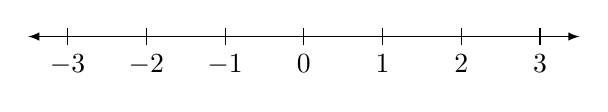
\begin{tikzpicture}
    \draw[latex-latex] (-3.5,0) -- (3.5,0) ; %edit here for the axis
    \foreach \x in  {-3,-2,-1,0,1,2,3} % edit here for the vertical lines
    \draw[shift={(\x,0)},color=black] (0pt,3pt) -- (0pt,-3pt);
    \foreach \x in {-3,-2,-1,0,1,2,3} % edit here for the numbers
    \draw[shift={(\x,0)},color=black] (0pt,0pt) -- (0pt,-3pt) node[below] 
    {$\x$};
    \end{tikzpicture}
\end{center}

\subsection{Conjunto Racional}
\begin{tcolorbox}[colback=yellow!5!white,colframe=yellow!50!black,
    colbacktitle=yellow!75!black,title={Definición - Conjunto Racional}]
    \[\mathbb{Q} \rightarrow \text{Conjunto de todas las fracciones } \frac{a}{b} \text{ donde } a \text{, } b \in \mathbb{Z} \text{ y } b \neq 0 \text{.}\]
    \[\mathbb{Q} = \bigl\{\frac{a}{b} : a \in \mathbb{Z}, b \in \mathbb{Z} - \{0\} \bigl\} \]
\end{tcolorbox}

\begin{center}
    \Large{
        $\text{M} 
        \in 
        \mathbb{N} 
        \Rightarrow 
        \frac{a}{b}$ = $\frac{a \cdot M}{b \cdot M}$
    }
\end{center}

\begin{tcolorbox}[colback=blue!5!white,colframe=blue!50!black,
    colbacktitle=blue!75!black,title={Fracciones equivalentes}]
    \[\frac{a}{b} = \frac{c}{d} \text{ si y solo si } a \cdot d = b \cdot c \]
\end{tcolorbox}

\paragraph{Operaciones con racionales}
\begin{itemize}
    % \textbf{Suma: \Rightarrow } $\frac{a}{b} \text{+} \frac{c}{b} \text{=} \frac{a+c}{b}$
    \item {\textbf{Suma: } \Large{$\frac{a}{b} + \frac{c}{b} = \frac{a+c}{b}$}}
    \item {\textbf{Multiplicación: } \Large{$\frac{a}{b} \cdot \frac{c}{d} = \frac{a \cdot c}{b \cdot d}$}}
    \item {\textbf{División: } \Large{$\frac{a}{b} : \frac{c}{d} = \frac{a}{b} \cdot \frac{d}{c} = \frac{a \cdot d}{b \cdot c}$}}
        
\end{itemize}

\end{document}
